\documentclass[11pt,a4paper]{article}

% ============================================================
% Paper Q1 (versi Bahasa Indonesia) — draft kerja
% NIDS Robust Lintas-Jaringan via Semantic Feature Mapping
% CSE-CIC-IDS2018 x UNSW-NB15 + evaluasi adversarial adaptif
% CATATAN: seluruh angka berasal dari eksperimen NYATA (T3-T9),
%          disimpan di unswnb-15/*.json. Bukan angka ilustratif.
% ============================================================

\usepackage[utf8]{inputenc}
\usepackage[T1]{fontenc}
\usepackage[bahasa]{babel}
\usepackage{graphicx}
\usepackage{booktabs}
\usepackage{amsmath,amssymb}
\usepackage{siunitx}
\usepackage{hyperref}
\usepackage{geometry}
\usepackage{caption}
\usepackage{multirow}
\geometry{margin=2.5cm}
\graphicspath{{figure-q1/}}

\hypersetup{colorlinks=true, linkcolor=blue, citecolor=blue, urlcolor=blue}

\title{\textbf{Menuju NIDS Robust Lintas-Jaringan: Pemetaan Fitur Semantik,
Adaptasi Domain Berbiaya-Rendah, dan Evaluasi Adversarial yang Realistis}}

\author{Hero Yudo Martono\thanks{Penulis koresponden: \texttt{hero@pens.ac.id}},
\quad Iwan Syarif, \quad Ferry Astika Saputra \\[0.3em]
\textit{Departemen Teknik Informatika, Politeknik Elektronika Negeri Surabaya,
Surabaya, Indonesia} \\
\texttt{hero@pens.ac.id; iwanarif@pens.ac.id; ferryas@pens.ac.id}}

\date{Draft --- \today}

\begin{document}
\maketitle

\begin{abstract}
Sistem deteksi intrusi jaringan (NIDS) berbasis pembelajaran mesin mencapai
akurasi tinggi ketika dilatih dan diuji pada jaringan yang sama, namun
kemampuannya untuk digeneralisasi lintas-jaringan jarang diuji secara jujur.
Makalah ini menyelidiki tiga masalah yang saling berkaitan pada NIDS praktis:
(1) ketidakmampuan generalisasi lintas-jaringan, (2) ketidaksepadanan fitur
antar-alat ekstraksi (\emph{feature-extractor mismatch}), dan (3) kerentanan
terhadap serangan \emph{evasion} adaptif. Menggunakan pasangan dataset
CSE-CIC-IDS2018 (68 fitur, CICFlowMeter) dan UNSW-NB15 (42 fitur, Argus/Bro)
yang diekstraksi dengan alat berbeda dari sumber trafik berbeda, kami menyusun
\emph{Semantic Feature Mapping} (SFM) yang divalidasi secara statistik untuk
memperoleh himpunan fitur irisan yang benar-benar sepadan. Kami menemukan bahwa
model XGBoost tunggal yang unggul di dalam-jaringan (MCC $0{,}91$ pada CIC;
$0{,}74$ pada UNSW) \emph{runtuh} lintas-jaringan (MCC $\approx 0$). Melalui
serangkaian eksperimen terkontrol, kami menunjukkan bahwa (i) \emph{adversarial
training} memperkuat ketahanan terhadap \emph{evasion} di dalam-jaringan tetapi
\emph{tidak} menutup celah generalisasi lintas-jaringan; (ii) celah tersebut
berakar pada \emph{distribution shift}, bukan ketidakcukupan fitur, sebab
pelatihan gabungan mencapai performa mendekati in-domain pada kedua jaringan
sekaligus; dan (iii) kalibrasi minimal --- hanya \emph{1\%} label jaringan
target, atau \emph{mixup} lintas-dataset tanpa label target sama sekali ---
memulihkan MCC lintas-jaringan ke rentang $0{,}65$--$0{,}91$. Terakhir, dengan
memberlakukan \emph{functional-preserving constraint} pada serangan, kami
menunjukkan bahwa evaluasi adversarial tak-terbatas melebih-lebihkan ancaman,
sementara evaluasi \emph{adaptive white-box} mengungkap bahwa \emph{adversarial
training} memberikan rasa aman yang keliru: pertahanan yang tampak kuat terhadap
serangan transfer (MCC $0{,}99$) runtuh terhadap penyerang adaptif
(MCC $0{,}25$--$0{,}43$). Temuan-temuan ini, seluruhnya berbasis eksperimen
nyata dan dilaporkan apa adanya, memberikan panduan yang jujur untuk merancang
dan mengevaluasi NIDS yang tangguh di dunia nyata.

\vspace{0.5em}
\noindent\textbf{Kata kunci:} sistem deteksi intrusi jaringan, generalisasi
lintas-jaringan, pemetaan fitur semantik, adaptasi domain, serangan adversarial
adaptif, XGBoost.
\end{abstract}

% ============================================================
\section{Pendahuluan}
\label{sec:intro}

NIDS berbasis pembelajaran mesin telah menjadi komponen penting pertahanan
siber, dan dievaluasi luas pada dataset \emph{benchmark} publik seperti KDD~Cup~99,
NSL-KDD, UNSW-NB15~\cite{unsw}, dan CIC-IDS2017/CSE-CIC-IDS2018~\cite{cicids}.
Namun sebagian besar evaluasi bertumpu pada protokol \emph{latih-dan-uji pada
dataset yang sama}, sehingga melaporkan akurasi yang optimistis dan tidak
mencerminkan kondisi penyebaran (\emph{deployment}) nyata. Dalam praktik, model
yang dilatih pada satu lingkungan jaringan harus beroperasi pada lingkungan lain
dengan topologi, komposisi trafik, dan alat ekstraksi fitur yang berbeda. Studi
generalisasi lintas-dataset yang mulai bermunculan~\cite{cantone,aceto}
menegaskan bahwa performa NIDS turun tajam ketika diuji lintas-dataset, namun
jarang mengisolasi \emph{penyebab} penurunan (fitur vs distribusi) atau menawarkan
solusi berbiaya-rendah yang tervalidasi.

Makalah ini merupakan kelanjutan langsung dari penelitian NIDS sebelumnya pada
CSE-CIC-IDS2018 (reduksi fitur XGBoost~\cite{xgboost} + \emph{adversarial
training} berbasis \emph{saliency map} + validasi \emph{real-traffic} AWS), yang
secara jujur mengakui tiga keterbatasan. Ketiga keterbatasan itulah yang menjadi
\textbf{gap inti} makalah ini:
\begin{enumerate}
  \item \textbf{Ketidakmampuan generalisasi lintas-jaringan.} Model kolaps saat
  menghadapi karakteristik trafik dari topologi jaringan berbeda.
  \item \textbf{Feature-extractor mismatch.} Perbedaan definisi fitur antar-alat
  ekstraksi (CICFlowMeter vs Argus/Bro) merusak akurasi pada inferensi nyata.
  \item \textbf{Kerentanan evasion adaptif.} \emph{Adversarial training}
  konvensional umumnya hanya dievaluasi terhadap serangan statis/transfer
  (grey-box), bukan penyerang \emph{white-box} yang menyesuaikan diri.
\end{enumerate}

\paragraph{Kontribusi.} Kontribusi makalah ini adalah:
\begin{itemize}
  \item \textbf{Semantic Feature Mapping (SFM)} lintas-dataset yang divalidasi
  secara statistik, termasuk temuan \emph{feature-extractor mismatch} pada fitur
  TCP window (Bagian~\ref{sec:sfm}).
  \item \textbf{Bukti kuantitatif} bahwa NIDS single-source runtuh
  lintas-jaringan, dan \textbf{pemisahan empiris} antara
  \emph{adversarial-robustness} dan \emph{cross-network-robustness} sebagai dua
  masalah berbeda (Bagian~\ref{sec:baseline},~\ref{sec:advtrain}).
  \item \textbf{Diagnosis} bahwa celah lintas-jaringan berakar pada
  \emph{distribution shift}, dan \textbf{solusi berbiaya-rendah}: kalibrasi
  minimal $1\%$ label target atau \emph{mixup} lintas-dataset
  (Bagian~\ref{sec:align},~\ref{sec:da}).
  \item \textbf{Metodologi evaluasi adversarial yang realistis}:
  \emph{functional-preserving evasion} dan \emph{adaptive white-box} yang
  mengoreksi klaim ketahanan yang berlebihan (Bagian~\ref{sec:fpe},~\ref{sec:awb}).
\end{itemize}

\paragraph{Prinsip kejujuran data.} Seluruh angka pada makalah ini bersumber
dari eksperimen nyata yang dapat direproduksi; tidak ada angka ilustratif yang
disamarkan sebagai hasil. Termasuk pelaporan jujur bahwa pertahanan kami sendiri
belum sepenuhnya tahan terhadap serangan adaptif.

% ============================================================
\section{Karya Terkait}
\label{sec:related}

\paragraph{NIDS berbasis pembelajaran mesin.} Model berbasis pohon (mis.
XGBoost~\cite{xgboost}) dan jaringan saraf dalam banyak dipakai pada dataset
\emph{benchmark}~\cite{unsw,cicids}. Mayoritas melaporkan hasil \emph{in-domain}
(latih-uji pada dataset sama) dengan akurasi tinggi, tetapi kondisi ini tidak
menjamin ketangguhan pada trafik jaringan yang berbeda dari data latih.

\paragraph{Generalisasi lintas-dataset.} Cantone \emph{et al.}~\cite{cantone}
melakukan studi generalisasi lintas-dataset sistematis (CIC-IDS2017,
CSE-CIC-IDS2018, dan variannya) dan menemukan penurunan performa yang konsisten
antar-dataset; Aceto \emph{et al.}~\cite{aceto} menyoroti peran sumber trafik dan
generator sintetik pada lintas-dataset. Studi-studi ini menegaskan adanya masalah,
namun umumnya berhenti pada pengamatan penurunan --- belum memisahkan kontribusi
\emph{ketidakcukupan fitur} versus \emph{pergeseran distribusi}, dan belum
menawarkan pemulihan berbiaya-rendah. Makalah kami mengisisi celah ini dengan
diagnosis terkontrol dan solusi kalibrasi minimal.

\paragraph{Adaptasi domain.} CORAL~\cite{coral} menyelaraskan statistik orde-2
(kovarians) antar-domain, sedangkan pendekatan berbasis MMD menyelaraskan momen
distribusi; pada data \emph{tabular} jaringan penerapan dan evaluasinya masih
terbatas. Pendekatan \emph{few-shot} juga mulai dieksplorasi untuk NIDS
data-terbatas~\cite{fewshot}. Kami mengevaluasi CORAL, pelatihan gabungan
(\emph{joint}), \emph{few-shot}, dan \emph{mixup} lintas-dataset secara langsung
pada pasangan CIC-IDS2018 dan UNSW-NB15.

\paragraph{Serangan adversarial pada NIDS.} Banyak karya menerapkan serangan
\emph{evasion} berbasis gradien atau GAN pada fitur alir~\cite{randhawa,mbow}
tanpa memperhatikan validitas protokol, sehingga menghasilkan \emph{flow} yang
tak dapat dikirim di jaringan nyata. Selain itu, evaluasi ketangguhan seringkali
hanya \emph{transfer}/grey-box, bukan \emph{adaptive white-box}, sehingga
berisiko melebih-lebihkan ketahanan --- fenomena \emph{obfuscated
gradients}~\cite{obfuscated} dan pentingnya \emph{adaptive
attacks}~\cite{adaptive} telah dibahas pada domain adversarial ML umum. Makalah
ini menutup kedua celah tersebut pada domain NIDS tabular lintas-jaringan:
serangan dibatasi \emph{functional-preserving} dan dievaluasi secara
\emph{adaptive white-box}.

% ============================================================
\section{Data dan Semantic Feature Mapping}
\label{sec:sfm}

\subsection{Dataset}
Kami memakai pasangan yang sengaja \emph{berbeda sumber}:
\begin{itemize}
  \item \textbf{CSE-CIC-IDS2018}: trafik \emph{testbed} CIC (2018), diekstraksi
  dengan CICFlowMeter, 68 fitur bersih. Label multi-kelas (Benign + 14 jenis
  serangan); untuk tahap ini digabung menjadi biner (attack/normal).
  \item \textbf{UNSW-NB15}: trafik dibangkitkan IXIA PerfectStorm (2015),
  diekstraksi dengan Argus \& Bro/Zeek, 42 fitur, 10 kelas. Berkas partisi:
  $175{.}341$ record (dipakai sebagai data latih) dan $82{.}332$ record (data
  uji).\footnote{Penamaan berkas rilis UNSW tertukar dengan isinya; kami memakai
  berkas berdasarkan jumlah record, bukan nama.}
\end{itemize}
Perbedaan alat ekstraksi dan sumber trafik ini bukan kelemahan, melainkan justru
prasyarat untuk menguji tiga gap inti secara jujur.

\subsection{Penyusunan dan Validasi Pemetaan}
SFM memetakan fitur berfungsi-sama antar-dataset meski bernama kolom berbeda
(mis. \texttt{Flow Duration}$\leftrightarrow$\texttt{dur}). Karena alat ekstraksi
berbeda, setiap pasangan kandidat divalidasi secara statistik (rentang,
distribusi, satuan) sebelum dipakai, bukan sekadar berdasarkan kemiripan nama.

\paragraph{Temuan kunci: TCP window mismatch.} Pemeriksaan nilai unik
membuktikan \texttt{swin}/\texttt{dwin} pada UNSW bersifat praktis biner
($\{0, 255\}$), sedangkan \texttt{Init Fwd/Bwd Win Byts} pada CIC kontinu
($0$--$65535$). Meski deskripsi resmi menyebut keduanya ``TCP window'', datanya
tidak sepadan. Kami \emph{membuang} pasangan ini dan melaporkannya sebagai studi
kasus \emph{feature-extractor mismatch} (gap \#2).

\subsection{Himpunan Fitur Final dan Pra-pemrosesan}
Kami memakai StandardScaler (z-score) \emph{per dataset terpisah} sehingga
perbedaan satuan/skala ternormalisasi tanpa mengarang konversi. Fitur final
(\textbf{Model A}, 9 fitur irisan kuat): \texttt{dur, spkts, dpkts, sbytes,
dbytes, smean, dmean, sload, dload}. \textbf{Model B} menambahkan
\texttt{sinpkt, dinpkt} (Fwd/Bwd IAT). Model A dipilih sebagai basis karena
setara Model B namun lebih ringkas.

\subsection{Pilihan Model Tunggal XGBoost: Perspektif \emph{Edge} dan \emph{Green AI}}
\label{sec:edge}
Kami sengaja mempertahankan \textbf{model tunggal XGBoost} alih-alih
\emph{ensemble} berat atau \emph{deep learning} kompleks. Selain menjaga
\emph{comparability} dengan penelitian sebelumnya dan mengisolasi variabel
kontribusi (SFM dan adaptasi lintas-jaringan, bukan kapasitas model), pilihan ini
selaras dengan kebutuhan \textbf{penyebaran di \emph{edge}} dan prinsip
\textbf{\emph{Green AI}}. Pada perangkat \emph{edge} nyata --- \emph{smart router},
\emph{IoT gateway}, atau sensor \emph{inline} --- model \emph{ensemble} multi-algoritma
atau jaringan dalam berukuran besar tidak realistis karena konsumsi memori, CPU,
dan energi yang tinggi, serta latensi inferensi yang dapat melampaui laju
kedatangan \emph{flow}. Sebaliknya, XGBoost tunggal dengan $9$ fitur menghasilkan
model biner ringan dan inferensi bertingkat-pohon yang cepat, menjadikannya
kandidat \emph{Edge-friendly Robust NIDS}.

\begin{table}[h]
\centering
\caption{Profil efisiensi Model A (9 fitur), diukur nyata pada satu inti CPU
(\emph{single-thread}, meniru \emph{edge} 1 vCPU).}
\label{tab:efficiency}
\begin{tabular}{lc}
\toprule
Metrik & Nilai \\
\midrule
Ukuran model biner (Model A, 9 fitur, 200 pohon) & $2{,}9$ MB \\
Rata-rata latensi inferensi per \emph{flow} (batch$=1$) & $\approx 439\ \mu$s \\
\emph{Throughput} inferensi (1 vCPU, inkremental) & $\approx 2\,276$ \emph{flow}/detik \\
\bottomrule
\end{tabular}
\end{table}

\noindent Angka pada Tabel~\ref{tab:efficiency} berasal dari pengukuran nyata
(XGBoost \emph{single-thread}, batch$=1$; median $434\ \mu$s, std $23\ \mu$s atas
$\sim$2000 \emph{flow}). Model $2{,}9$ MB (200 pohon, kedalaman 8) cukup ringkas
untuk dimuat pada perangkat \emph{edge}, dan laju $>2\,000$ \emph{flow}/detik per
satu inti memadai untuk banyak titik pemantauan jaringan --- mendukung klaim
\emph{Edge-friendly}. Kami melaporkan angka apa adanya: latensi berorde ratusan
mikrodetik (bukan puluhan), dan menghindari pelaporan \emph{throughput} \emph{batch}
yang dapat menyesatkan akibat optimasi vektorisasi.

% ============================================================
\section{Baseline Lintas-Dataset: Celah Generalisasi}
\label{sec:baseline}

Kami melatih XGBoost (\texttt{max\_depth}=8, \texttt{lr}=0{,}1,
\texttt{n\_estimators}=200, \texttt{subsample}/\texttt{colsample}=0{,}8) dan
mengevaluasi empat skenario. Metrik utama MCC (tahan \emph{class imbalance}).

Verifikasi label dilakukan: pada CIC \texttt{Benign}$=0$; konversi biner
menghasilkan tepat $1{.}348{.}453$ normal dan $274{.}808$ attack, sehingga MCC
negatif lintas-jaringan adalah fenomena nyata, bukan artefak label.

\begin{table}[h]
\centering
\caption{Baseline lintas-dataset (MCC, Model A). Performa in-domain tinggi namun
lintas-jaringan runtuh.}
\label{tab:baseline}
\begin{tabular}{lcc}
\toprule
Skenario & Model A & Model B \\
\midrule
Same-CIC (latih \& uji CIC)   & $0{,}913$ & $0{,}914$ \\
Same-UNSW (latih \& uji UNSW) & $0{,}745$ & $0{,}743$ \\
CIC$\rightarrow$UNSW          & $-0{,}072$ & $0{,}004$ \\
UNSW$\rightarrow$CIC          & $-0{,}061$ & $-0{,}046$ \\
\midrule
\emph{Generalization gap}     & $0{,}81$--$0{,}99$ & $0{,}79$--$0{,}91$ \\
\bottomrule
\end{tabular}
\end{table}

\begin{figure}[h]
\centering
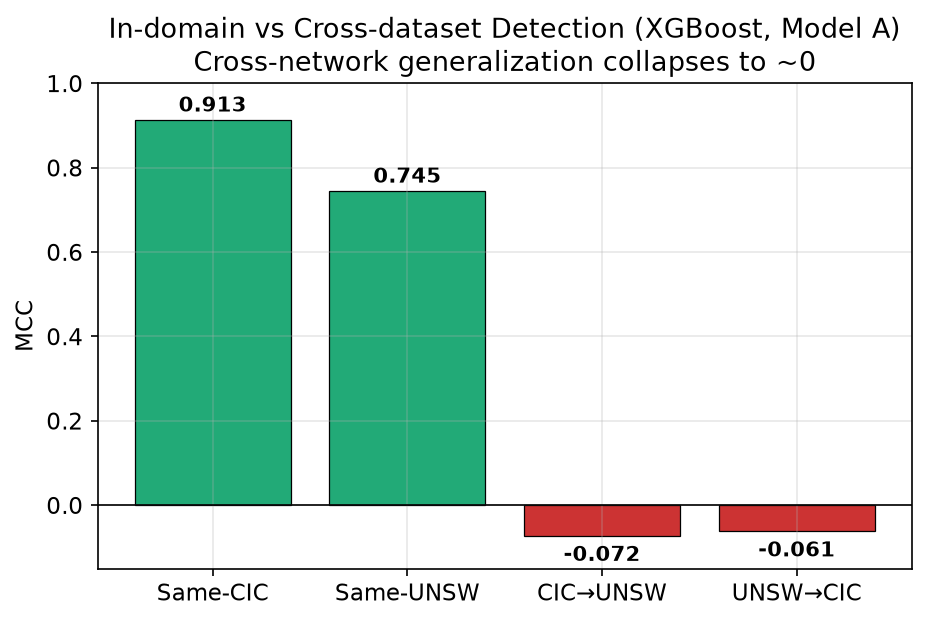
\includegraphics[width=0.72\linewidth]{fig1_generalization_gap.png}
\caption{Deteksi in-domain vs lintas-dataset. Model yang unggul di dalam-jaringan
jatuh ke MCC $\approx 0$ lintas-jaringan.}
\label{fig:gap}
\end{figure}

Tabel~\ref{tab:baseline} dan Gambar~\ref{fig:gap} menunjukkan bahwa MCC $\approx 0$
(setara tebakan acak) hingga negatif lintas-jaringan. Ini bukti empiris gap \#1.

% ============================================================
\section{Adversarial Training Tidak Menutup Celah Lintas-Jaringan}
\label{sec:advtrain}

Kami menerapkan \emph{adversarial training} bergaya makalah sebelumnya. Karena
XGBoost berbasis pohon dan \emph{non-differentiable}, gradien loss terhadap fitur
tidak tersedia secara analitik. Kami mengestimasinya dengan skema
\emph{central finite-difference}: untuk setiap fitur ke-$i$,
\begin{equation}
\label{eq:fd}
\widehat{\left[\nabla_{\mathbf{x}} L(\theta,\mathbf{x},y)\right]}_i
\;=\;
\frac{L\!\left(\theta,\mathbf{x}+h\,\mathbf{e}_i,\,y\right)
      - L\!\left(\theta,\mathbf{x}-h\,\mathbf{e}_i,\,y\right)}{2h},
\qquad i=1,\dots,d,
\end{equation}
dengan $\mathbf{e}_i$ vektor basis satuan pada dimensi ke-$i$, $h$ langkah kecil
($h=0{,}01$ pada ruang ter-\emph{z-score}), $d$ jumlah fitur, dan $L$ \emph{binary
cross-entropy}
$L(\theta,\mathbf{x},y) = -\bigl[y\log p_\theta(\mathbf{x}) + (1-y)\log(1-p_\theta(\mathbf{x}))\bigr]$,
$p_\theta(\mathbf{x})$ probabilitas kelas \emph{attack}. Estimasi
Persamaan~\eqref{eq:fd} memerlukan $2d$ evaluasi model per sampel.

Sampel adversarial dibangkitkan dengan \emph{Fast Gradient Sign Method} (FGSM),
\begin{equation}
\label{eq:fgsm}
\mathbf{x}_{adv} \;=\; \mathbf{x} + \epsilon\,\mathrm{sign}\!\left(\widehat{\nabla_{\mathbf{x}} L(\theta,\mathbf{x},y)}\right),
\end{equation}
lalu model diperkuat melalui augmentasi $D_{robust}=D_{clean}\cup D_{adv}$ dengan
rasio $80{:}20$ dan dilatih ulang. Formulasi ini setara dengan pendekatan
\emph{min-max} (\emph{saddle-point}) $\min_\theta \mathbb{E}\bigl[\max_{\|\boldsymbol{\delta}\|_\infty \le \epsilon} L(\theta,\mathbf{x}+\boldsymbol{\delta},y)\bigr]$,
dengan $\max$ dalam diaproksimasi oleh FGSM satu langkah.

Hasilnya \emph{asimetris terhadap tujuan}: robustness \emph{evasion} in-domain
membaik tajam (MCC $-0{,}09 \rightarrow +0{,}36$ pada $\epsilon=0{,}1$),
\emph{tetapi} MCC lintas-jaringan tetap $\approx 0$ (CIC$\rightarrow$UNSW
$-0{,}072 \rightarrow -0{,}011$; UNSW$\rightarrow$CIC $-0{,}061 \rightarrow
-0{,}066$). Ini memisahkan secara empiris \emph{adversarial-robustness} dari
\emph{cross-network-robustness}: keduanya masalah berbeda dan memerlukan solusi
berbeda.

% ============================================================
\section{Diagnosis: Celah Berakar pada \emph{Distribution Shift}}
\label{sec:align}

Kami membandingkan tiga strategi (Tabel~\ref{tab:align},
Gambar~\ref{fig:align}): \emph{baseline} single-source, \emph{CORAL}
(\emph{unsupervised domain adaptation}, penyelarasan kovarians source$\rightarrow$
target), dan \emph{joint training} (gabungan CIC+UNSW, uji test masing-masing).

\begin{table}[h]
\centering
\caption{Strategi penyelarasan lintas-jaringan (MCC pada target).}
\label{tab:align}
\begin{tabular}{lcc}
\toprule
Strategi & CIC$\rightarrow$UNSW & UNSW$\rightarrow$CIC \\
\midrule
Baseline single-source & $-0{,}072$ & $-0{,}061$ \\
CORAL (unsup. DA)      & $-0{,}185$ & $+0{,}164$ \\
Joint training (uji test) & \multicolumn{2}{c}{UNSW $0{,}732$ \quad CIC $0{,}912$} \\
\bottomrule
\end{tabular}
\end{table}

\begin{figure}[h]
\centering
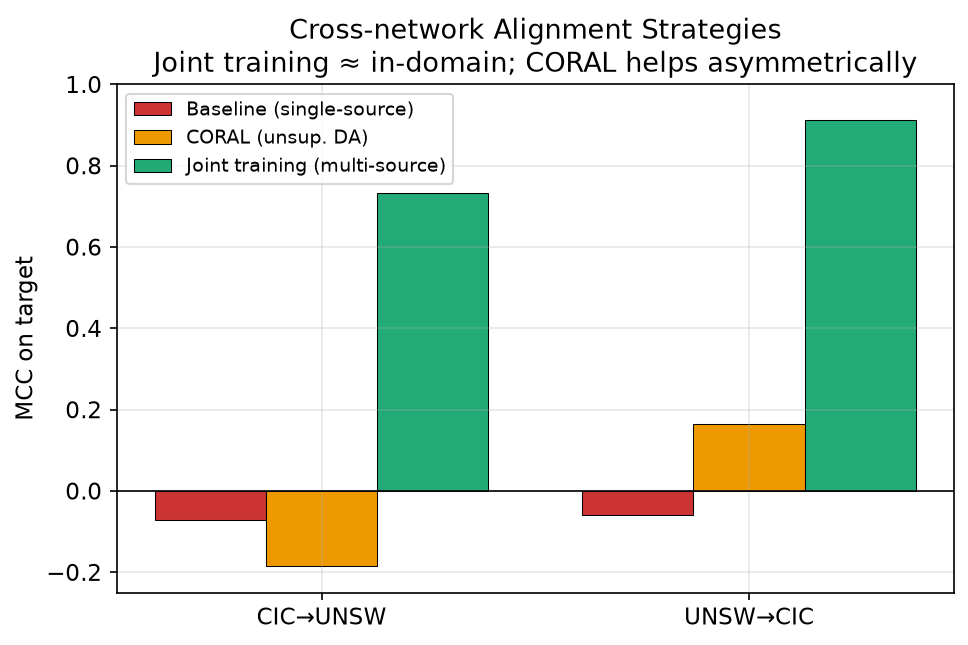
\includegraphics[width=0.72\linewidth]{fig3_alignment.png}
\caption{Strategi penyelarasan. Joint training mencapai $\approx$ in-domain pada
kedua jaringan; CORAL membantu asimetris.}
\label{fig:align}
\end{figure}

Temuan terpenting: \emph{joint training} mencapai MCC $0{,}912$ (CIC) dan
$0{,}732$ (UNSW) \emph{serentak}, hampir setara in-domain. Ini membuktikan
\textbf{SFM valid} --- 9 fitur irisan cukup ekspresif merepresentasikan kedua
jaringan. Maka celah generalisasi \emph{bukan} pada fitur, melainkan pada
\emph{distribution shift}: model single-source tak melihat distribusi target.
CORAL membantu sebagian dan asimetris (UNSW$\rightarrow$CIC naik ke $+0{,}164$;
CIC$\rightarrow$UNSW malah turun), menandakan penyelarasan orde-2 belum memadai
untuk arah dari sumber berdistribusi kaya.

% ============================================================
\section{Solusi Berbiaya-Rendah: Kalibrasi Minimal dan \emph{Mixup}}
\label{sec:da}

Karena celah bersifat \emph{distribution shift}, kami menguji \emph{few-shot
target adaptation}: melatih pada source ditambah fraksi kecil label target
($0/1/5/10/25\%$; fraksi diambil dari \emph{train} target, uji di \emph{test}
target tanpa kebocoran). Sebagai pembanding tanpa label target, kami memakai
\emph{cross-dataset mixup} (interpolasi Beta antar-\emph{flow} kedua dataset).

\begin{table}[h]
\centering
\caption{Few-shot target adaptation (MCC lintas-jaringan).}
\label{tab:fewshot}
\begin{tabular}{lcc}
\toprule
Fraksi label target & CIC$\rightarrow$UNSW & UNSW$\rightarrow$CIC \\
\midrule
$0\%$ (baseline)  & $-0{,}072$ & $-0{,}061$ \\
$1\%$             & $0{,}648$  & $0{,}899$  \\
$5\%$             & $0{,}662$  & $0{,}911$  \\
$10\%$            & $0{,}681$  & $0{,}911$  \\
$25\%$            & $0{,}695$  & $0{,}912$  \\
\midrule
Mixup (tanpa label target) & $0{,}680$ & $0{,}798$ \\
\bottomrule
\end{tabular}
\end{table}

\begin{figure}[h]
\centering
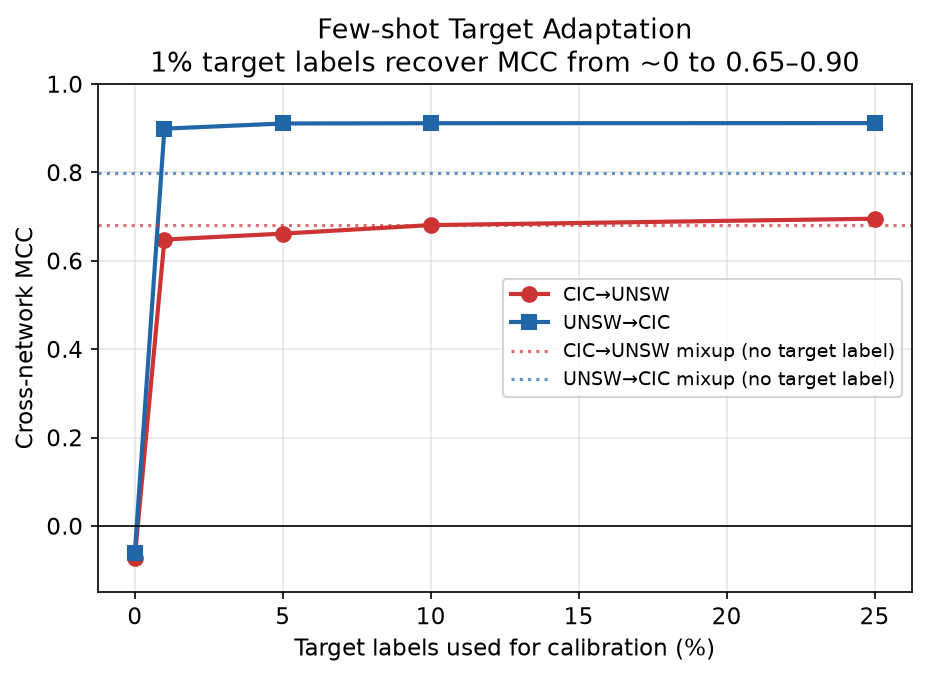
\includegraphics[width=0.72\linewidth]{fig2_fewshot_curve.png}
\caption{Kurva few-shot. Hanya $1\%$ label target memulihkan MCC dari negatif ke
$0{,}65$--$0{,}90$; kurva mendatar setelahnya.}
\label{fig:fewshot}
\end{figure}

Tabel~\ref{tab:fewshot} dan Gambar~\ref{fig:fewshot} menunjukkan lompatan
dramatis: hanya $1\%$ label target ($1{.}753$ \emph{flow} UNSW atau $11{.}362$
\emph{flow} CIC) membalik MCC dari negatif menjadi $0{,}648$ (CIC$\rightarrow$UNSW)
dan $0{,}899$ (UNSW$\rightarrow$CIC, mendekati in-domain $0{,}913$). Setelah
$1\%$ kurva mendatar, sehingga \emph{kalibrasi minimal sudah cukup}. \emph{Mixup}
tanpa label target pun mencapai $0{,}680$ dan $0{,}798$. Pesan praktis: berkat
SFM, NIDS lintas-jaringan dapat dibuat berfungsi dengan sedikit --- atau tanpa
--- label dari jaringan baru.

% ============================================================
\section{Evaluasi Adversarial yang Realistis}

\subsection{Functional-Preserving Evasion}
\label{sec:fpe}

FGSM tak-terbatas (Persamaan~\eqref{eq:fgsm}) dapat menghasilkan \emph{flow}
mustahil (paket pecahan, \emph{bytes} $<$ paket, durasi negatif) yang tak dapat
dikirim di jaringan nyata. Kami merumuskan serangan sebagai \emph{constrained
optimization}: penyerang mencari perturbasi yang memaksimalkan loss namun tetap
berada di dalam \emph{ruang perturbasi layak} $\mathcal{S}_{valid}(\mathbf{x})$,
\begin{equation}
\label{eq:fpe-opt}
\mathbf{x}_{adv} \;=\; \arg\max_{\mathbf{x}' \in \mathcal{S}_{valid}(\mathbf{x})}\;
L\!\left(\theta,\mathbf{x}',y\right),
\qquad
\|\mathbf{x}' - \mathbf{x}\|_\infty \le \epsilon .
\end{equation}
Misalkan fitur dinyatakan pada ruang asli (bukan ter-\emph{z-score}). Ruang
$\mathcal{S}_{valid}$ didefinisikan oleh himpunan kendala protokol/fisik berikut:
\begin{subequations}
\label{eq:constraints}
\begin{align}
x'_j &\ge 0, && \forall j \ \text{(non-negatif: durasi, volume, laju)}, \label{eq:c-nonneg}\\
x'_j &\in \mathbb{Z}^{+}, && j \in \{spkts,\, dpkts\} \ \text{(jumlah paket bulat)}, \label{eq:c-int}\\
sbytes' &\ge spkts', \quad dbytes' \ge dpkts', && \text{(tiap paket} \ge 1 \ \text{byte)}, \label{eq:c-consistency}\\
smean' &= \tfrac{sbytes'}{spkts'}, \quad dmean' = \tfrac{dbytes'}{dpkts'}, && \text{(konsistensi rata-rata)}, \label{eq:c-mean}\\
x'_j &\ge x_j, && j \in \{spkts, dpkts, sbytes, dbytes, dur\} \ \text{(monotonic \emph{add-only})}. \label{eq:c-mono}
\end{align}
\end{subequations}
Kendala~\eqref{eq:c-mono} mencerminkan keterbatasan penyerang nyata: ia hanya
dapat \emph{menambah} trafik (padding, paket sisipan), tidak dapat mengurangi
paket/byte yang sudah terkirim. Untuk fitur biner/kategori, batas langkah
efektif $\delta = 0$ (tak boleh diubah). Secara operasional, kami memakai
\emph{projected FGSM}: langkah FGSM Persamaan~\eqref{eq:fgsm} diikuti proyeksi
$\Pi_{\mathcal{S}_{valid}}(\cdot)$ yang menerapkan Persamaan~\eqref{eq:constraints}
di ruang asli sebelum dipetakan kembali ke ruang ter-\emph{z-score}.

Operator proyeksi $\Pi_{\mathcal{S}_{valid}}$ didefinisikan secara operasional
sebagai komposisi terurut berikut. Diberikan sampel kandidat $\mathbf{x}'$ pada
ruang ter-\emph{z-score} dan \emph{scaler} per-dataset $(\boldsymbol{\mu},
\boldsymbol{\sigma})$:
\begin{enumerate}
  \item \textbf{Denormalisasi:} $\mathbf{u} \leftarrow \mathbf{x}' \odot
  \boldsymbol{\sigma} + \boldsymbol{\mu}$ (ke ruang fitur asli).
  \item \textbf{Non-negatif:} $u_j \leftarrow \max(u_j, 0)$ untuk semua $j$
  [Pers.~\eqref{eq:c-nonneg}].
  \item \textbf{Pembulatan paket:} $u_j \leftarrow \operatorname{round}(u_j)$
  untuk $j\in\{spkts, dpkts\}$ [Pers.~\eqref{eq:c-int}].
  \item \textbf{Monotonic \emph{add-only}:} $u_j \leftarrow \max(u_j, x^{\text{orig}}_j)$
  untuk $j\in\{spkts, dpkts, sbytes, dbytes, dur\}$, dengan $\mathbf{x}^{\text{orig}}$
  sampel bersih acuan [Pers.~\eqref{eq:c-mono}].
  \item \textbf{Konsistensi volume:} $sbytes \leftarrow \max(sbytes, spkts)$;
  $dbytes \leftarrow \max(dbytes, dpkts)$ [Pers.~\eqref{eq:c-consistency}].
  \item \textbf{Penyetelan rata-rata:} $smean \leftarrow sbytes/spkts$ bila
  $spkts>0$ (analog untuk $dmean$), menjaga identitas statistik
  [Pers.~\eqref{eq:c-mean}].
  \item \textbf{Renormalisasi:} $\Pi_{\mathcal{S}_{valid}}(\mathbf{x}') \leftarrow
  (\mathbf{u} - \boldsymbol{\mu}) \oslash \boldsymbol{\sigma}$ (kembali ke ruang
  ter-\emph{z-score}).
\end{enumerate}
Urutan langkah penting: penegakan \emph{add-only} (4) mendahului konsistensi
volume (5) dan penyetelan rata-rata (6) agar hasil akhir memenuhi seluruh kendala
secara simultan. Fitur biner/kategori (tidak dipakai pada Model A) memiliki
$\delta=0$ sehingga dilewati proyeksi.

\begin{figure}[h]
\centering
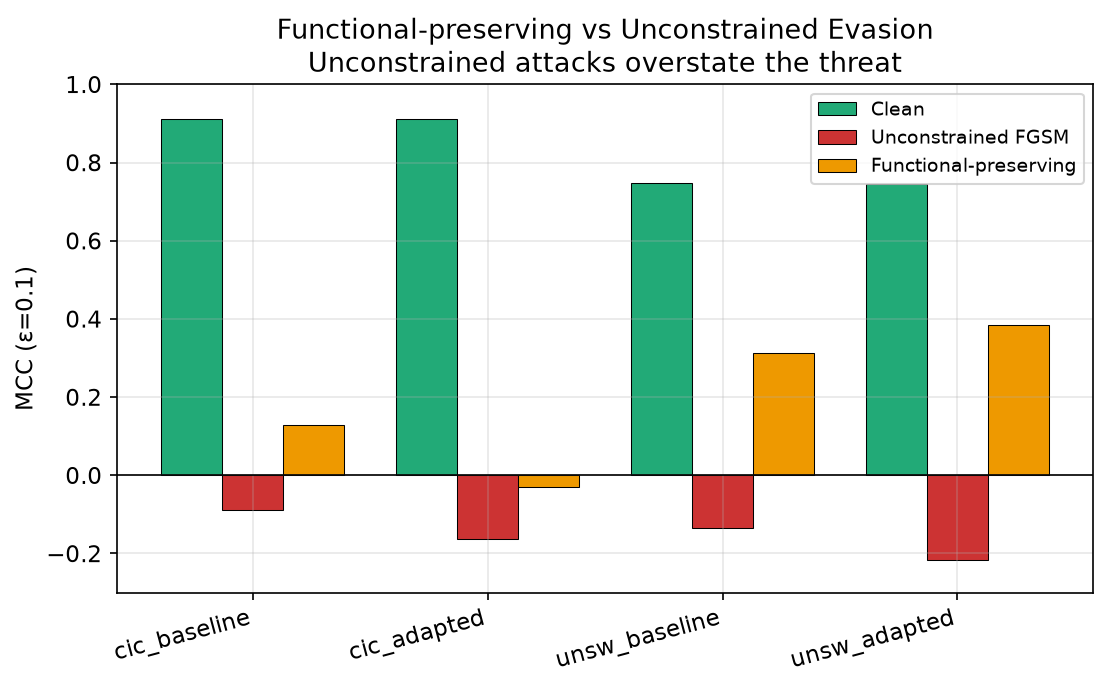
\includegraphics[width=0.82\linewidth]{fig4_functional_evasion.png}
\caption{Evasion \emph{functional-preserving} vs tak-terbatas ($\epsilon=0{,}1$).
Serangan tak-terbatas melebih-lebihkan ancaman.}
\label{fig:fpe}
\end{figure}

Pada keempat model (Gambar~\ref{fig:fpe}), MCC \emph{functional} jauh di atas
\emph{unconstrained} (mis. UNSW baseline $-0{,}134 \rightarrow +0{,}313$),
membuktikan evaluasi tak-terbatas melebih-lebihkan ancaman. Namun MCC
\emph{functional} tetap turun tajam dari kondisi bersih (CIC $0{,}912 \rightarrow
0{,}127$), sehingga ancaman \emph{flow} valid tetap nyata.

\subsection{Adaptive White-Box}
\label{sec:awb}

Skenario terburuk: penyerang mengetahui model pertahanan dan membangkitkan
\emph{evasion} langsung dari gradien model \emph{robust} itu sendiri (bukan
transfer dari baseline). Seluruh serangan tetap \emph{functional-preserving}.

\begin{table}[h]
\centering
\caption{Adaptive white-box (MCC model \emph{robust}, $\epsilon=0{,}1$).}
\label{tab:awb}
\begin{tabular}{lccc}
\toprule
Arah & Bersih & Serangan transfer & Serangan adaptif \\
\midrule
CIC  & $0{,}911$ & $0{,}993$ & $0{,}425$ \\
UNSW & $0{,}733$ & $0{,}985$ & $0{,}248$ \\
\bottomrule
\end{tabular}
\end{table}

\begin{figure}[h]
\centering
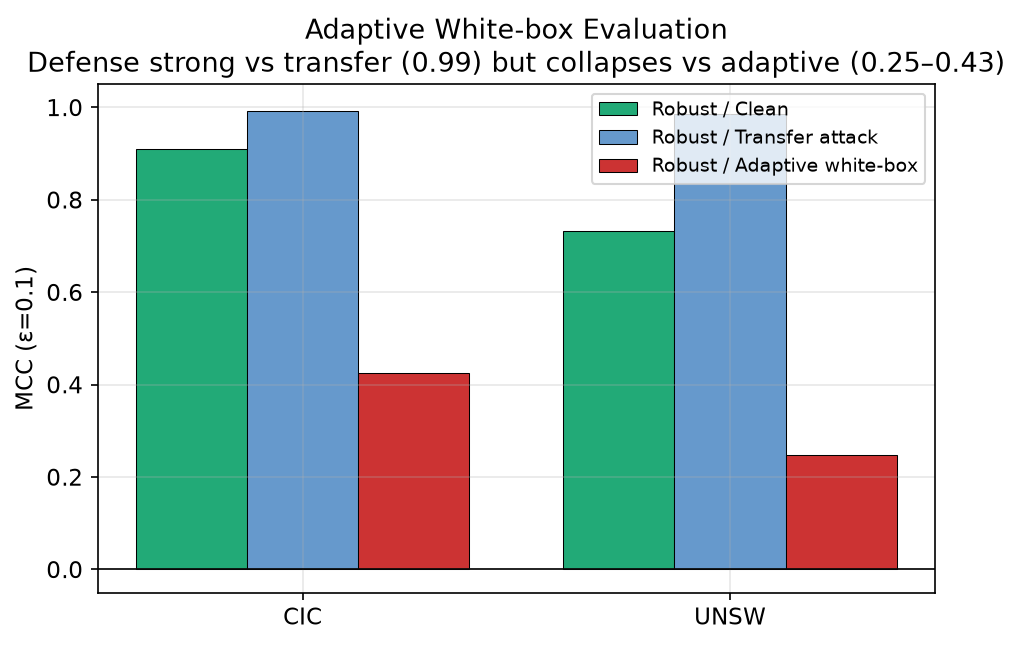
\includegraphics[width=0.72\linewidth]{fig5_adaptive_whitebox.png}
\caption{Evaluasi \emph{adaptive white-box}. Pertahanan kuat terhadap transfer
($0{,}99$) namun runtuh terhadap penyerang adaptif ($0{,}25$--$0{,}43$).}
\label{fig:awb}
\end{figure}

Tabel~\ref{tab:awb} dan Gambar~\ref{fig:awb} mengungkap \emph{false robustness}:
model \emph{robust} tampak sangat kuat terhadap serangan transfer (MCC $0{,}99$)
tetapi runtuh terhadap penyerang adaptif (MCC $0{,}425$ pada CIC; $0{,}248$ pada
UNSW). Ini konsisten dengan fenomena \emph{obfuscated gradients}: model
``menghafal'' pola serangan transfer, bukan menjadi robust sejati. Konsekuensi
metodologis: evaluasi ketahanan NIDS \emph{wajib} menyertakan
\emph{adaptive white-box}; laporan yang hanya \emph{transfer} menyesatkan.

\paragraph{Arah mitigasi (kerja mendatang).} Temuan ini tidak berhenti pada
pengungkapan kelemahan. Beberapa strategi menjanjikan untuk memperkuat ketahanan
terhadap serangan adaptif dapat dieksplorasi: (i) \emph{adversarial training}
berbasis \emph{multi-step} PGD dengan \emph{functional-preserving constraint}
diterapkan sejak fase pelatihan (bukan FGSM satu langkah), sehingga model
menghadapi perturbasi terkuat-yang-valid alih-alih menghafal satu pola transfer;
dan (ii) \emph{randomized smoothing} atau penghalusan batas keputusan
(\emph{decision-boundary smoothing}) yang mengaburkan sinyal gradien pada model
berbasis pohon, menyulitkan penyerang mengoptimasi arah \emph{evasion}. Kedua
pendekatan ini merupakan arah lanjutan yang wajar bagi NIDS tabular.

% ============================================================
\section{Diskusi}
\label{sec:discussion}

Rangkaian temuan membentuk narasi yang koheren dan jujur:
(1) NIDS single-source runtuh lintas-jaringan;
(2) penyebabnya bukan \emph{evasion} dan bukan fitur, melainkan
\emph{distribution shift};
(3) kalibrasi minimal atau \emph{mixup} memulihkan performa secara efisien
berkat SFM yang tervalidasi;
(4) evaluasi adversarial harus realistis (functional-preserving) dan
menyeluruh (adaptive white-box), jika tidak akan melebih-lebihkan ketahanan.

\subsection{Analisis Asimetri Performa Adaptasi}
\label{sec:asymmetry}
Sebuah pola konsisten muncul di seluruh eksperimen adaptasi: arah
CIC$\rightarrow$UNSW selalu memulihkan MCC lebih rendah
($\sim 0{,}65$--$0{,}70$ pada few-shot; $-0{,}185$ pada CORAL) dibandingkan arah
UNSW$\rightarrow$CIC ($\sim 0{,}90$ pada few-shot; $+0{,}164$ pada CORAL). Kami
menganalisis asimetri ini dari sudut \textbf{kompleksitas domain}.

CSE-CIC-IDS2018 dibangkitkan pada infrastruktur \emph{testbed} yang relatif
terstruktur, sedangkan UNSW-NB15 dibangkitkan dengan generator IXIA
PerfectStorm yang menyuntikkan variasi serangan lebih beragam
(sembilan kelas: \emph{Fuzzers, Analysis, Backdoors, DoS, Exploits, Generic,
Reconnaissance, Shellcode, Worms}) dengan tingkat \emph{noise} lebih tinggi.
Akibatnya, distribusi UNSW-NB15 pada ruang fitur irisan lebih ``lebar'' dan
heterogen. Memindahkan model dari domain \emph{sederhana} (CIC) ke domain
\emph{kompleks} (UNSW) secara inheren lebih sulit: model sumber tidak pernah
melihat mode-mode distribusi kaya milik target. Sebaliknya, memindahkan dari
domain kompleks (UNSW) ke domain lebih terstruktur (CIC) lebih mudah karena
target merupakan himpunan bagian perilaku yang sebagian sudah tercakup.

Interpretasi ini konsisten dengan dua bukti internal: (i) CORAL --- yang
menyelaraskan kovarians orde-2 --- justru \emph{memperburuk} arah
CIC$\rightarrow$UNSW ($-0{,}072 \rightarrow -0{,}185$) karena memaksa struktur
sumber yang sempit menutupi ruang target yang lebih luas; dan (ii) pelatihan
gabungan (\emph{joint}) tetap menyisakan selisih (UNSW $0{,}732$ vs CIC $0{,}912$),
menandakan sebagian kompleksitas UNSW sulit direpresentasikan oleh $9$ fitur
irisan meskipun kedua domain terlihat saat pelatihan. Asimetri ini karena itu
merupakan properti struktural pasangan dataset, bukan artefak metode.

\paragraph{Keterbatasan.} Kami melaporkan secara jujur bahwa pertahanan
\emph{adversarial training} kami belum tahan terhadap serangan adaptif; asimetri
arah CIC$\rightarrow$UNSW ($\sim 0{,}65$--$0{,}70$) vs UNSW$\rightarrow$CIC
($\sim 0{,}91$) juga belum sepenuhnya teratasi (dianalisis pada
\S\ref{sec:asymmetry}). Evaluasi masih terbatas pada tugas biner. Penggunaan
model tunggal XGBoost adalah \emph{pilihan desain} yang disengaja demi efisiensi
\emph{edge} (\S\ref{sec:edge}), bukan sekadar keterbatasan; eksplorasi
\emph{ensemble} robust ditinggalkan sebagai arah lanjutan yang harus tetap
mempertimbangkan anggaran komputasi penyebaran.

% ============================================================
\section{Kesimpulan dan Kerja Mendatang}
\label{sec:conclusion}

Kami menyajikan studi lintas-jaringan yang jujur pada pasangan CSE-CIC-IDS2018
dan UNSW-NB15. \emph{Semantic Feature Mapping} yang tervalidasi memungkinkan
pelatihan lintas-dataset; kami menunjukkan bahwa celah generalisasi berakar pada
\emph{distribution shift} dan dapat ditutup dengan kalibrasi berbiaya-rendah
($1\%$ label target) atau \emph{mixup} tanpa label. Kami juga mengoreksi praktik
evaluasi adversarial melalui \emph{functional-preserving} dan
\emph{adaptive white-box}.

\paragraph{Kerja mendatang.} (i) Klasifikasi multi-kelas dan model
\emph{ensemble} robust dengan tetap mempertimbangkan anggaran komputasi
\emph{edge}; (ii) adaptasi domain yang lebih kuat untuk mengatasi asimetri arah;
(iii) pertahanan yang benar-benar tahan \emph{adaptive white-box};
(iv) \emph{deployment} jangka panjang di AWS ($3$--$7$ hari) untuk mengukur
\emph{False Alarm Rate} pada trafik nyata.

Gambar~\ref{fig:deploy} menyajikan \emph{blueprint} arsitektur penyebaran yang
kami rencanakan: trafik langsung (\emph{VPC mirror}/ENI) ditangkap oleh sensor
EC2 yang menjalankan NFStream untuk mengekstraksi fitur \emph{flow}, diselaraskan
melalui SFM dan \emph{z-score}, lalu diinferensikan oleh model XGBoost \emph{robust}
ringan untuk deteksi \emph{real-time} sekaligus pencatatan FAR. \emph{Blueprint}
ini menunjukkan kesiapan teknis untuk validasi lanjutan tersebut.

\begin{figure}[h]
\centering
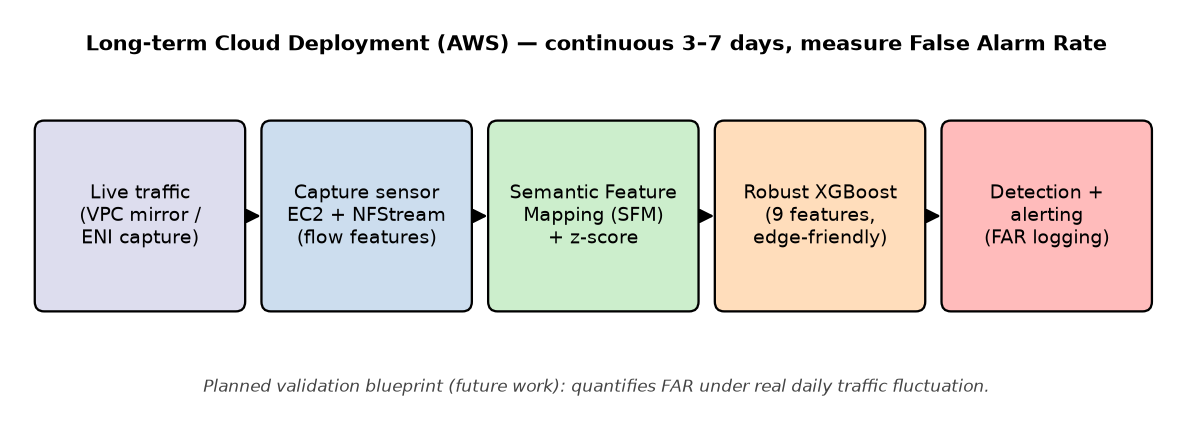
\includegraphics[width=0.98\linewidth]{fig6_deployment_blueprint.png}
\caption{\emph{Blueprint} penyebaran jangka panjang di AWS (rencana kerja
mendatang): pipeline sensor$\rightarrow$SFM$\rightarrow$XGBoost robust untuk
mengukur \emph{False Alarm Rate} pada trafik nyata $3$--$7$ hari.}
\label{fig:deploy}
\end{figure}

% ============================================================
\section*{Ketersediaan Reproduksi}
Kode, konfigurasi, \emph{notebook}, dan berkas hasil ringkas ($*.json$) tersedia
di repositori. Dataset besar tidak disertakan (lisensi/ukuran) namun dapat
diperoleh dari sumber resmi masing-masing.

% Format referensi: gaya IEEE — inisial nama depan; judul dalam tanda kutip;
% nama venue italik; konferensi diawali "in Proc."; halaman & tahun.
\begin{thebibliography}{9}
\bibitem{coral} B.~Sun, J.~Feng, and K.~Saenko, ``Return of frustratingly easy
domain adaptation,'' in \emph{Proc. 30th AAAI Conf. Artificial Intelligence
(AAAI)}, Phoenix, AZ, USA, 2016, pp.~2058--2065.

\bibitem{obfuscated} A.~Athalye, N.~Carlini, and D.~Wagner, ``Obfuscated
gradients give a false sense of security: Circumventing defenses to adversarial
examples,'' in \emph{Proc. 35th Int. Conf. Machine Learning (ICML)}, Stockholm,
Sweden, 2018, pp.~274--283.

\bibitem{adaptive} F.~Tram\`er, N.~Carlini, W.~Brendel, and A.~M\k{a}dry, ``On
adaptive attacks to adversarial example defenses,'' in \emph{Proc. 34th Conf.
Neural Information Processing Systems (NeurIPS)}, Vancouver, Canada, 2020,
pp.~1633--1645.

\bibitem{unsw} N.~Moustafa and J.~Slay, ``UNSW-NB15: A comprehensive data set
for network intrusion detection systems (UNSW-NB15 network data set),'' in
\emph{Proc. Military Communications and Information Systems Conf. (MilCIS)},
Canberra, Australia, 2015, pp.~1--6.

\bibitem{cicids} I.~Sharafaldin, A.~H.~Lashkari, and A.~A.~Ghorbani, ``Toward
generating a new intrusion detection dataset and intrusion traffic
characterization,'' in \emph{Proc. 4th Int. Conf. Information Systems Security
and Privacy (ICISSP)}, Funchal, Portugal, 2018, pp.~108--116.

\bibitem{xgboost} T.~Chen and C.~Guestrin, ``XGBoost: A scalable tree boosting
system,'' in \emph{Proc. 22nd ACM SIGKDD Int. Conf. Knowledge Discovery and
Data Mining (KDD)}, San Francisco, CA, USA, 2016, pp.~785--794.

\bibitem{cantone} M.~Cantone, C.~Marrocco, and A.~Bria, ``Machine learning in
network intrusion detection: A cross-dataset generalization study,'' \emph{IEEE
Access}, vol.~12, pp.~144491--144509, 2024.

\bibitem{aceto} G.~Aceto, F.~Giampaolo, C.~Guida, S.~Izzo, A.~Pescap\`e,
F.~Piccialli, and E.~Prezioso, ``Synthetic and privacy-preserving traffic trace
generation using generative AI models for training network intrusion detection
systems,'' \emph{J. Netw. Comput. Appl.}, vol.~229, art.~103926, 2024.

\bibitem{fewshot} C.~Xu, Y.~Zhan, G.~Chen, Z.~Wang, S.~Liu, and W.~Hu,
``Elevated few-shot network intrusion detection via self-attention mechanisms
and iterative refinement,'' \emph{PLoS ONE}, vol.~20, no.~1, art.~e0317713, 2025.

\bibitem{randhawa} R.~H.~Randhawa, N.~Aslam, M.~Alauthman, and H.~Rafiq,
``Evasion generative adversarial network for low data regimes,'' \emph{IEEE
Trans. Artif. Intell.}, vol.~4, no.~5, pp.~1076--1088, 2023.

\bibitem{mbow} M.~Mbow, R.~Roman, T.~Takahashi, and K.~Sakurai, ``Evading IoT
intrusion detection systems with GAN,'' in \emph{Proc. 19th Asia Joint Conf.
Information Security (AsiaJCIS)}, 2024, pp.~48--55.
\end{thebibliography}

\end{document}
